%\subsection{Background}

\section{Network traffic}\label{traffic}



Computers in a network mostly communicate by sending \textit{network packets} to each other, in which the transmitted information is encapsulated. Each network packet is split into the control information, also called packet header, and the user information, called payload. The packet header contains the necessary information for the correct transmission of the packet, including the transmission protocol layer (such as TCP, UDP, or ICMP), and the source and destination IP addresses and network ports\footnote{A network port is a number that identifies which service or application is responsible for the processing of incoming packets.}. It furthermore contains error-checking fields suchs as the size of the packet and a checksum over the payload, and protocol-specific fields. 


\begin{figure}[h!]
\centering
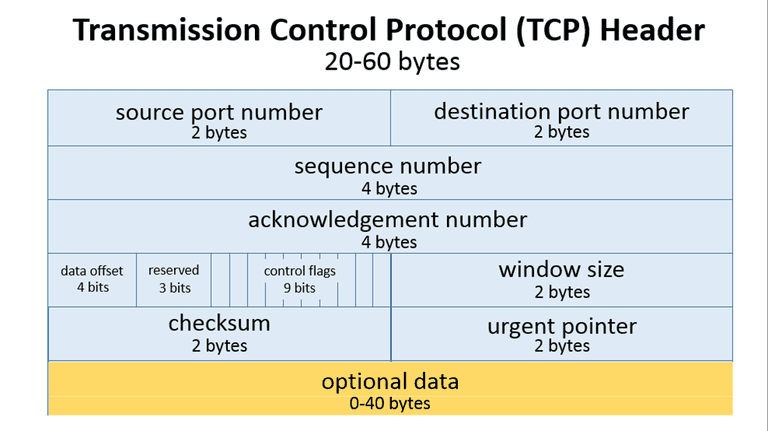
\includegraphics[scale=0.4]{images/tcp_header.png}
\caption{Typical format of a TCP packet. Source:\scriptsize{ https://www.lifewire.com/tcp-headers-and-udp-headers-explained-817970}\normalsize}
\end{figure}


The payload of a packet is in general the data that is carried on behalf of an application. It can be of variable length, however, it cannot exceed the maximum packet length set by the network protocol. In contrast to the packet header, the payload can be encrypted, a technique that makes it unreadable to any third parties and that is becoming increasingly common in modern computer networks. 


While traversing between to parties, a network packet can pass multiple connecting devices which direct the packet in the right direction. Any device in the immediate circuit traversed by a packet can capture and store it. In a monitoring setting, packets are usually captured by network routers and stored in the widespread \textit{pcap} format. In case of space shortage or privacy concerns, the payload of a packet can be dropped in the saving process.


Another more structured way of capturing network traffic is based on connection summaries, or \textbf{network flows}. RFC 3697 \cite{brownlee1999traffic} defines a network flow as a sequence of packets that share the same source and destination IP address, IP protocol, and for TCP and UDP connections the same source and destination port. A network flow is usually saved containing these informations along with the start and duration of the connection and the number of packets and bytes transferred in the connection.


\begin{figure}[h!]
\scriptsize
\centering
\begin{verbatim}
 Date flow start        Duration Proto  Src IP Addr:Port      Dst IP Addr:Port   Packets  Bytes Flows
 2010-09-01 00:00:00.459   0.000 UDP    127.0.0.1:24920   ->  192.168.0.1:22126      1     46     1
 2010-09-01 00:00:00.363   0.000 UDP    192.168.0.1:22126 ->  127.0.0.1:24920        1     80     1
\end{verbatim}
\normalsize
\caption{A typical network flow output}
\end{figure}


Raw packets grant full information about the connection, but take a lot of space when stored, whereas network flows give a more structured and lightweight overview over the traffic in a network. Both data formats are used widely by NIDSs.

\subsection{Network attacks}

Sophisticated data breaches affect hundreds of million customers and inflicts tremendous financial, reputational, and logistic damage. %Cyber-security incidents increased by 38\% in 2017, and the global cost of cyber crime is estimated to reach \$2 trillion by 2019 %\citep{conteh2016rise}. The prevention of cyber crime is therefore a globally demanded necessity.
One reason for the recent rise of cyber crime is the increased use of sophisticated techniques for the attack of specific targets. Attackers use customised social engineering and custom-build malware that penetrate defensive barriers and potentially stay undetected in an infected system for an extended period of time. 



%Existing solutions to commercial intrusion detection in computer networks are often based on \textbf{detecting signatures} of previously uncovered and analysed  attacks. Examples of such signatures include  file  hashes of malicious software, blacklisted IP addresses and domain names, and characteristics of known Command-and-Control (C\&C) protocols. Detection of a signature usually indicates an imminent intrusion and triggers investigation. 



%However, with attackers becoming adept at shedding such previously identified signatures, cyber-security researchers have to find ways of quantifying malicious activity in a more robust way. 

%However, attackers are becoming more adept at shedding previously gathered signatures: A file hash can be altered by minor modifications in the program and IP and domain addresses can be switched by changing servers. A sophisticated attack will employ new, customized protocols and software that is fitted to the targeted computer infrastructure, and thus will not show any identified signatures. 

%The field of \textit{Intrusion Detection} is concerned with the development of methods and tools that identify malicious behaviour in a computer network in a more robust way. %\textcolor{red}{In this work, I will discuss existing literature concerning a sub-branch intrusion detection, that is concerned with detecting anomalous behaviour in network traffic.... network intrusion detection  and anomaly detection}

In 1980, James P. Anderson, a member of the \textit{Defense Science Board Task Force on Computer Security} at the U.S. Air Force, published the first report to introduce the notion of automated intrusion detection \cite{anderson1980computer}. In it, he defines an \textbf{intrusion attempt} or a threat as 

\begin{quote}
\textit{"\dots an unauthorized and deliberate attempt to access or manipulate information, or to render a system unreliable or unusable."}
\end{quote}

Such attacks can be very diverse in their nature: They can be used to achieve different goals, and correspondingly exploit different types of tools and vulnerabilities. Very often, intrusive attacks involve some sort network communication between the victim machine(s) and a malicious agent. As this work is focusing primaly on network intrusion and corresponding defense systems, we will take a closer look at this type of communication. A recent survey covering intrusive attacks and defense systems distinguishes five classes of malicious network traffic \cite{nisioti2018intrusion}:

\begin{enumerate}
\item \textit{DoS-attacks}: A denial-of-service attack is an attempt to remove ability of a particular computer to communicate with other machines over an extended period of time. Such attacks are usually targeted at network servers in order to disrupt the service it is providing. All major types of DoS-attacks achieve this by overwhelming the target server with service requests, which are usually corrupted in a way that causes the server to bind resources unnessecarily long for each request, and thus losing its capability to process other requests. The most prominent type of DoS attacks are SYN-floods. They exploit the TCP-handshake protocol by sending many SYN-requests to a server while ignoring the SYN-ACK response packets sent in return by the server. This causes the server to keep waiting for a response for each of the attacker's requests, and thus binds the resources of the server while being computationally very cheap for the attacker. After a certain treshold, the server will not be able to process any more requests, rendering it unusable for actual client requests.

\item \textit{Network probing/Reconnaissance attack}: The purpose of network probing attacks is to gather information about computers in a network and possibly find vulnerabilities which can be exploited in further attacks. This typically involves sending specific service requests to other computers in the network in order to gather information about this system, such as open ports or the operating system running on a machine, contained in the corresponding response packets.

A common type of network probing attacks is \textit{port scanning}. Its aim is to gather knowledge of computers in the network than run vulnerable services, such as HTTP servers, mail servers, and so on. A port scan achieves this by sending queries to one or more network ports on one or more computers in the network. A computer on which the contacted network port is open will respond to the query and thus reveils himself. A port scan can either be vertical, during many ports on one computer are scanned, or horizontal, where the attacker scans a small number of ports on many computers in the network. 

Network probing is often an integral part in the spreading mechanism of\textit{computer worms}.

\item \textit{Access Attacks}: These are attacks that attempt to gain unauthorized access to a machine. This could both be an individual from outside gaining access to the network, or a user from inside the network accessing services or privileges outside of their authority. Access attacks are often divided into \textit{Remote-to-Local} (R2L) where a remote attacker gains access on a system over the network, and \textit{User-to-Root} (U2R), where a user illegally gains administrator access to a machine. However, many attacks fall into both categories. 

Access attacks can be very diverse in their nature. A simple example are brute-force attacks where an attacker guesses the passwort of a user over a network service such as SSH. Other prominent and more sophisticated cases include \textit{SQL injections}, where nefarious SQL statements are passed to an entry field for execution, or \textit{buffer overflow}, in which more data is put into a buffer of a service than it can hold in order manipulate data in the memory past the buffer.


\item \textit{Data Manipulation Attack}: Also known as "man-in-the-middle", these attacks typically involve an attacker reading and manipulating information in a data stream that is not addressed to him by exploiting vulnerable or missing authentication mechanisms in the IP protocol and related applications. A common form of such an exploit is \textit{IP spoofing} where an attacker pretends to be a trusted computer by sending packets with a spoofed trusted source IP address. Similarly, vulnerabilities in digital certificates that serve as a unique identifier of a trusted computer can be used to create fake certificate and thus trick a victim into trusting the intruder carrying the faked certificate.

Two examples of data manipulation attacks are \textit{session replay} and \textit{website impersonation}. In a session replay, the intruder captures packet sequences exchanged between two parties and modifies part of the data before forwarding it to the receiver. Here, both parties are unaware of the data manipulation and trust the authenticity of the connection. In website impersionation, a user is unknowingly redirected to a perfect copy of the website he requested. The user is then tricked to enter confidential information into a web form, which is then sent to the attacker instead of the trusted party operating the original page. 


Data manipulation attacks are often used pass malicious code to a victim in order to gain access on its machine. An impressive example of such behaviour was demonstrated by the malware \textit{Flame}\footnote{also known as \textit{Skywiper}}: An infected host in a network sends messages to other machines running Windows advertising itself as a Windows update provider, using spoofed IP addresses and a fake Microsoft certificate and thus defeating Microsoft's authentication mechanism. Other computers were consequently tricked into receiving malicious updates from the infected host, which would then infect their machine \cite{skywiperskywiper}.



\item \textit{C}\&\textit{C traffic}: 

C\& stands for \textit{"Command and Control"} and denotes the communication between an infected host and a rogue agent, called the C\&C server. The data transmitted in a C\&C channel is usually exfiltrated information about the environment of the infected host, or commands from the C\&C server for the victim for further operations. Typically, C\&C communication is used for the control of one or more so called \textit{bots}, computers that can perform tasks such as network scanning, establishing connections to other machines, or participating in DoS attacks. The communication between a bot and the C\&C server is therefore extended and continuous over time. However, C\&C communication can also be used for the request and transmission of an encryption key needed in a ransomware attack, in which it is limited in time and size. 

C\&C communication is usually sent over the HTTP or HTTPS protocol as it is widely available and allows the attacker to hide their communication in the large volume of diverse traffic sent over this channel \cite{lamprakis2017unsupervised}.

\end{enumerate}

An additional class of networking threats is the \textit{unauthorized surveillance} of network traffic. A local network of computers is usually separated from the outside, with a router establishing the connection between computers in the network and ones outside the network. The traffic exchanged between machines inside the network therefore does not leave the network and is not visible for outsiders. Unauthorised access captures of internal network traffic can give an intruder significant information about the network topology, and even access to sensitive information if a connection is not encrypted. As network surveillance usually does not leave any visible traces in the network, I did not include it in the above listed types of malicious traffic. 




\section{Machine learning and anomaly detection}

\subsection{Sequence modelling}

\subsection{Classification vs anomaly-detection}
Supervised vs self-supervised

\subsection{Self-supervised language models}

\section{Intrusion detection}

Sophisticated data breaches affect hundreds of million customers and inflict tremendous financial, reputational, and logistic damage. One reason for the recent rise of cyber crime is the increased use of advanced techniques for the attack of specific targets. Attackers use customised social engineering and custom-built malware that penetrate defensive barriers and potentially stay undetected in an infected system for an extended period of time. 

Cyber-security relies on a range of defensive techniques, including sophisticated intrusion detection systems and firewalls that try to detect and prevent attacks against software subsystems. Malicious software still remains the biggest threat to computer users, and its detection is of utmost importance. 

The field of intrusion detection is concerned with the development of methods and tools that identify and locate possible intrusions in a computer network. An \textit{intrusion detection system} (IDS) is typically a device or software application that detects malicious activity or policy violations in an automated way by scanning incoming data collected from one or more sources for patterns that a model or a set of rules classifies as potentially malicious.

Intrusion detection is a well researched area, with the first IDSs emerging in the late 1980's. Intrusion detection today comprises a variety of research areas in terms of different types of data sources, system architectures, detection sope, and so forth. Denning \cite{denning1987intrusion} in 1987 established the notion of two different types IDS implementations: a) host-based and b) network-based. 
\textit{Host-based intrusion detection systems} (HIDS) monitor each host in a network individually, and rely on local data streams such as application logs or raw operating system calls as  data source. \textit{Network-based intrusion detection} refers to the detection of malicious traffic in a network of computers and uses network traffic captures as a data source. In this PhD project, I will mainly focus on network traffic as a data source due its universal nature, its resilience against modification, and my previous experience in the field. However, I will also investigate the possibility of relating both types of traffic. For more details on IDS implementations, I refer the reader to my more detailed literature review. 


Current detection methods are predominantly based on the analysis of previously identified attack signatures, which provides great reliability and low false alert rates. However, these methods are dependent on an updated attack signature database and provide no protection against previously unseen attacks. With attackers having access to more resources than ever, custom built malware is becoming more common to circumvent signature-based detection. 

Another approach that has recently gained traction in commercial deployment is based on detecting malware and other undesired activity as anomalous behaviour when compared to benign computer activity. In this approach, known as \textbf{network anomaly detection} after Denning \cite{denning1987intrusion}, models must quantify the behaviour of normal network behaviour to be independent of a narrowly defined notion of malicious activity.

\subsection{Intrusion Detection Systems}

The field of intrusion detection is concerned with the development of methods and tools that identify and locate possible intrusions in a computer network. An \textit{intrusion detection system} (IDS) is typically a device or software application that detects malicious activity or policy violations in an automated way by scanning incoming data collected from one or more sources for patterns that a model or a set of rules classifies as malicious.

Intrusion detection is a well researched area, with the first IDSs emerging in the late 1980's. Intrusion detection today comprises a variety of research areas in terms of different types of data sources, system architectures, detection sope, and so forth. Figure \ref{graph} provides a broad yet uncomplete overview of these different areas. 

\subsubsection*{Implementation}

Denning \cite{denning1987intrusion} in 1987 established the notion of two different types IDS implementations: a) host-based and b) network-based. 
\textit{Host-based intrusion detection systems} (HIDS) monitor each host in a network individually, and rely on local data streams such as application logs or raw operating system calls as  data source. A relatively new form of host-based data sources are biometrik user data such as keystrokes or eye movement, please see \cite{peng_user_2016} for more information.

\textit{Network-based intrusion detection} refers to the detection of malicious traffic in a network of computers. A network intrusion detection system (NIDS) monitors network traffic within in a network and/or between the network and external hosts for malicious activity or policy violations. Network traffic data can take different forms, a more detailled explanation will be provided in Section \ref{traffic}.

\begin{figure}\label{graph}
\centering
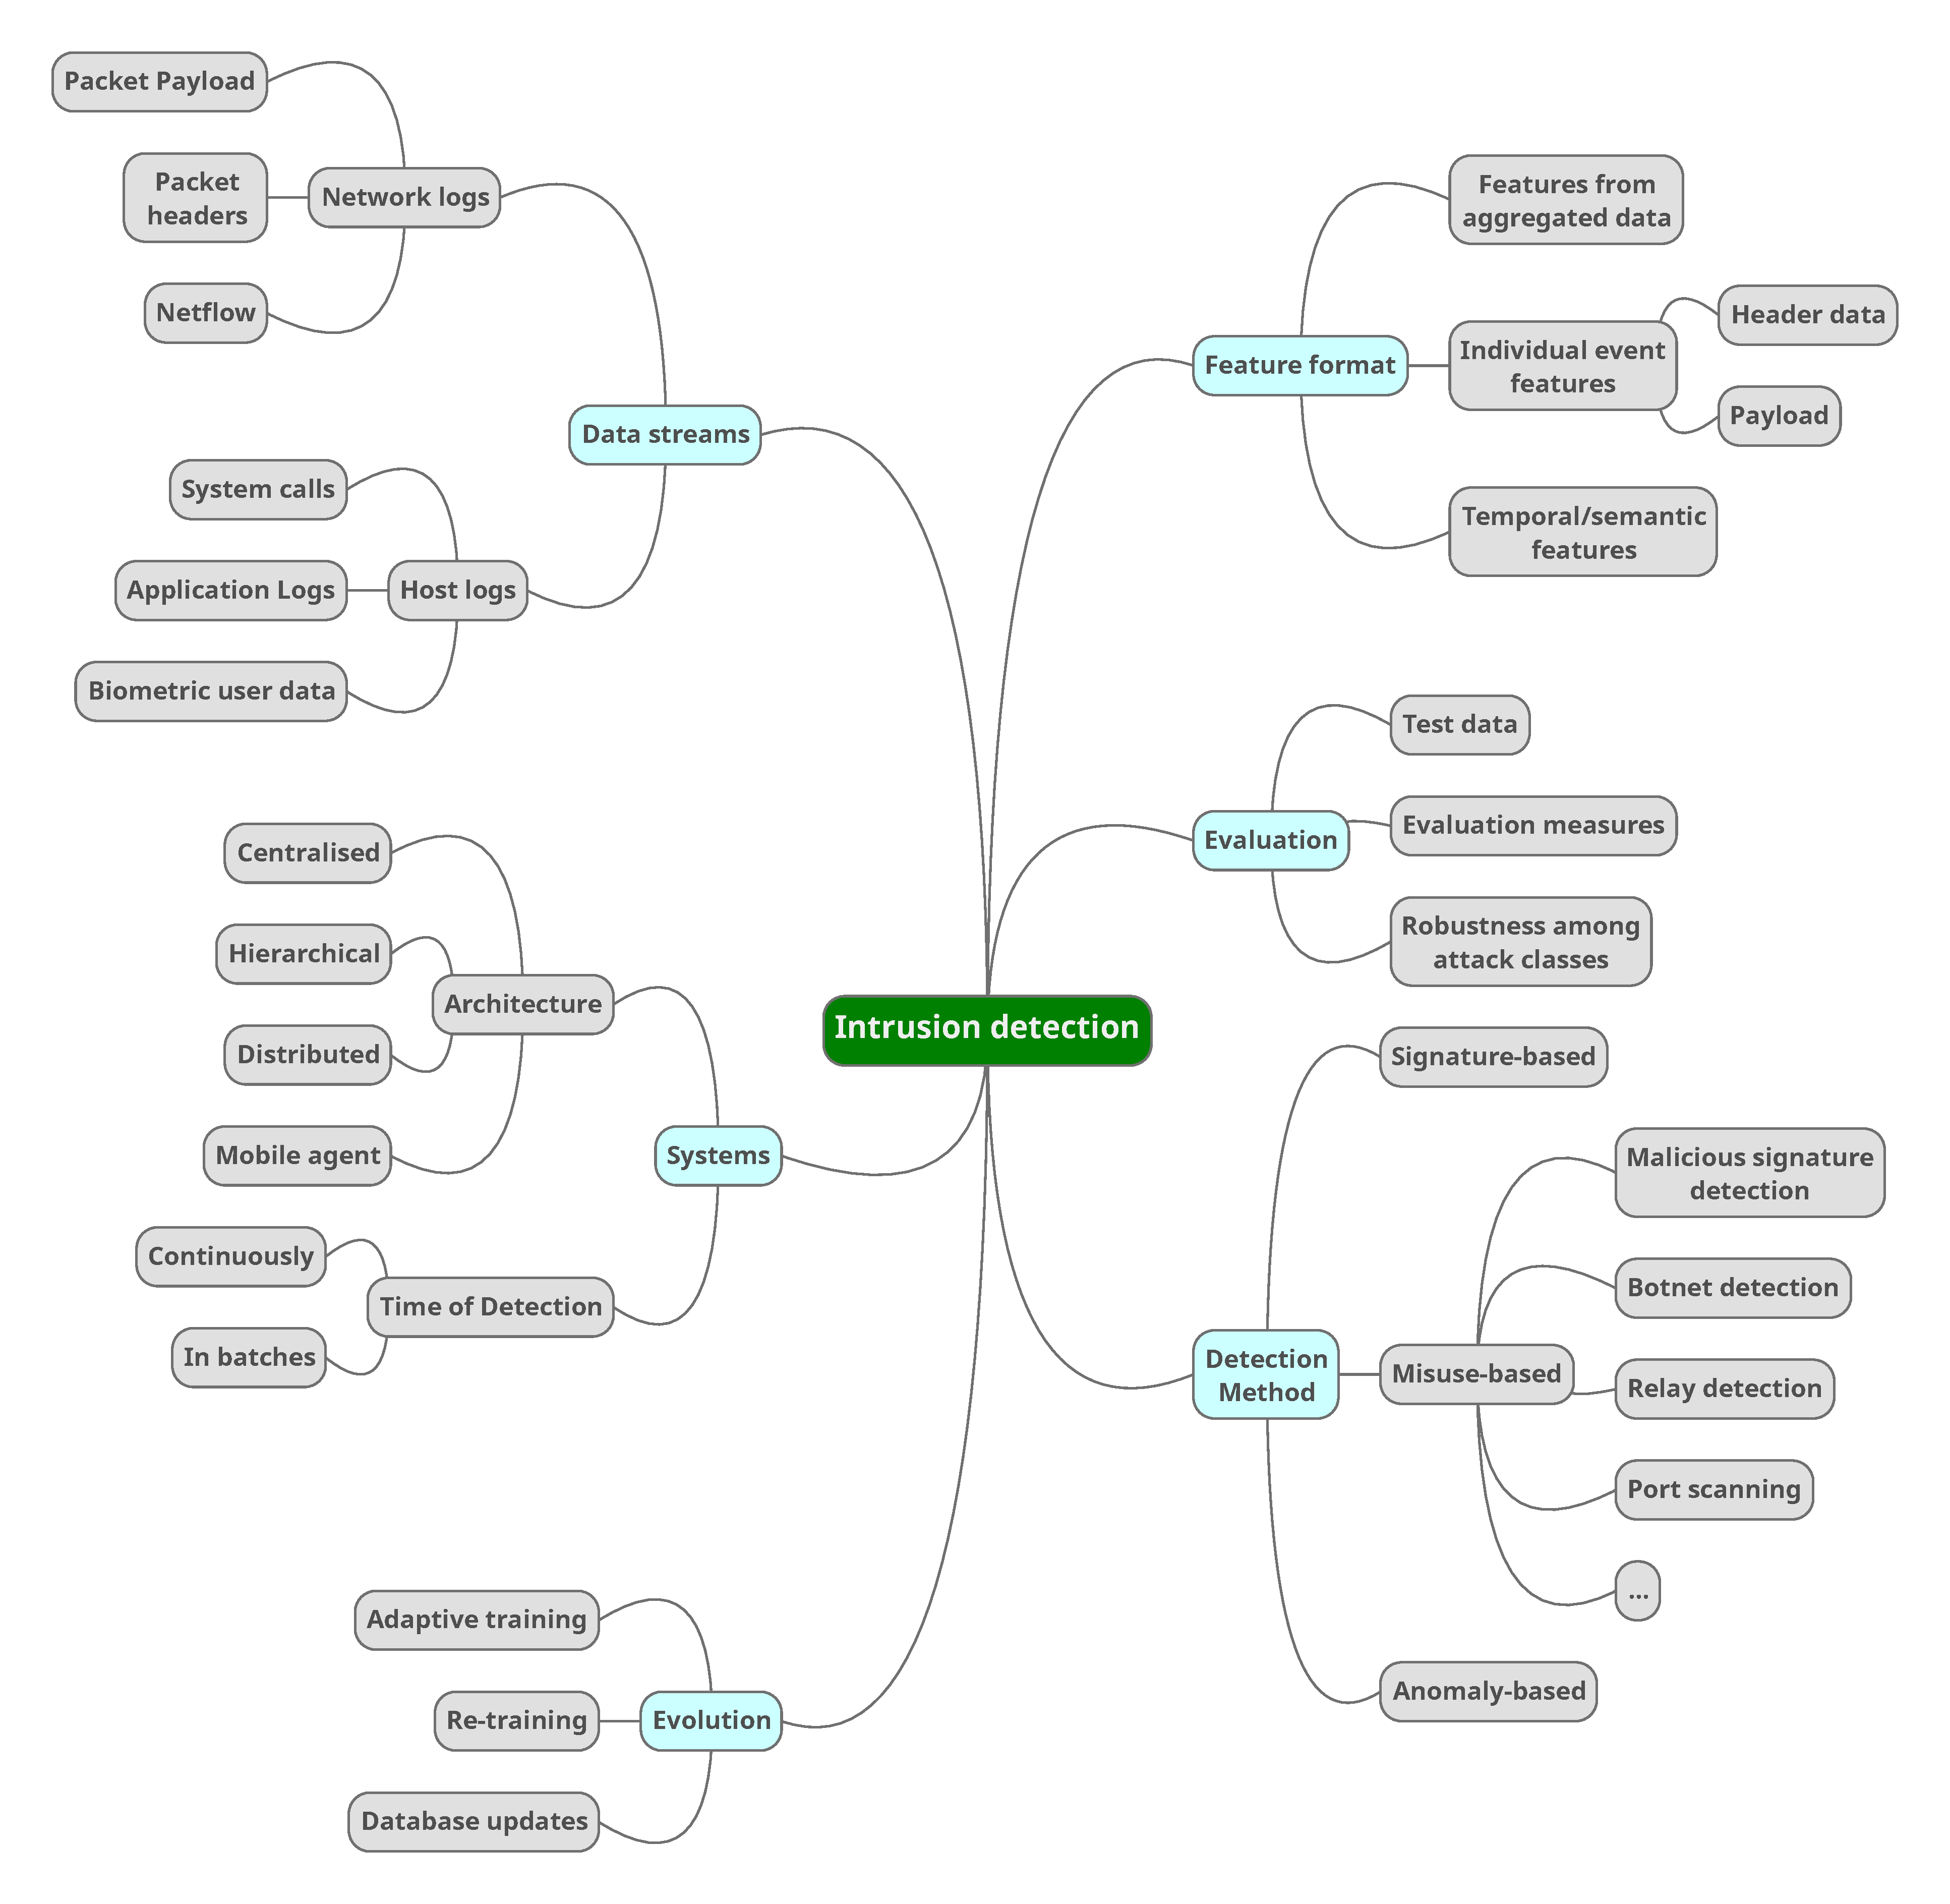
\includegraphics[scale=0.25]{images/Graphic2.pdf}
\caption{A broad overview over different aspects in an IDS}
\end{figure}

Host-based systems have the advantage of working with high quality data that   are   typically   very   informative \cite{lazarevic2005intrusion}. NIDS have the advantage of being plattform independent and more resiliant to attacks as detection of an infection is not done on the infected system. In this review, I will focus on work done in the area of network intrusion detection.


\subsubsection*{Detection methods}

Detection methods are the core of an IDS, and are therefore the most important design choice. Traditionally, two broad types of detection approaches are identified: a) Misuse detection and b) anomaly detection. 

Misuse detection aims at detecting a particular and well known reoccurring characteristic or pattern of a malicious behaviour. Two simple examples of such a characteristic are the large number of SYN packets sent by a host in a DoS attack, and the synchronised connection of many hosts to one server in a botnet. In misuse detection, abnormal or malicious behaviour is therefore defined first before developing a model to distinguish the defined behaviour from other traffic.

In contrast, anomaly detection aims at building a model of normal system behaviour that is accurate enough to spot any malicious behaviour as traffic that deviates from the estimated model. Anomaly detection is principally more difficult than misuse detection since the traffic model has to incorporate potentially very heterogenuous traffic behaviours. However, it is generally acknowledged that anomaly detectionhas is more suitable to detect new and previously unseen malicious behaviour as it makes no definite assumptions on the anomalous behaviour. Misuse detection is robust against evolution of malware as long as defined malicious behaviours do not change.

In reality, anomaly and misuse detection are not necessarily mutually exclusive, and there is a fluent passage between the two. This is because many anomaly detection approaches choose a particular set of features to be modelled with a particular threat in mind. For instance, models for the number of connections of a machine are naturally suitable for detecting DoS attacks, port scans, or Worm attacks. 

As misuse detection detection methods are aimed at detecting very specific behaviour, they usually only detect one type of malicious traffic. Areas that have been researched particularly well include botnet C\&C channel detection, DoS attack detection, and port scan detection. Areas that lack a comprehensive body of research are different types of R2L and U2R attacks. These are also currently the least   detected   attack   classes \cite{nisioti2018intrusion}.

\subsection{Anomaly detection}

Anomaly detection refers to the problem of identifying data instances that have significantly different properties than previously observed ``normal data instances. Anomaly detection has its origins in statistical research where normal data instances are assumed to be generated as random variables by a probability distribution $P_\textit{N}(X)$. New data is then identified as anomalous if its properties correspond to regions with vanishing likelihood, i.e. this particular data instance is highly unlikely to be generated by $P_\textit{N}(X)$. Usually, the hard part in anomaly detection is to use observed data efficiently to build an estimated distribution $\hat{P}_\textit{N}(X)$ that resembles $P_\textit{N}(X)$ closely to identify anomalous events while asigning normal instances a non-vanishing likelihood. A variety of techniques exist to achieve this assuming comparably simple generating distributions. However, distributions for many interesting types of normal data can be complex and changing over time, and individual data points can have intricate interdependencies. 
\begin{figure}
\centering
\begin{subfigure}[b]{0.45\textwidth}
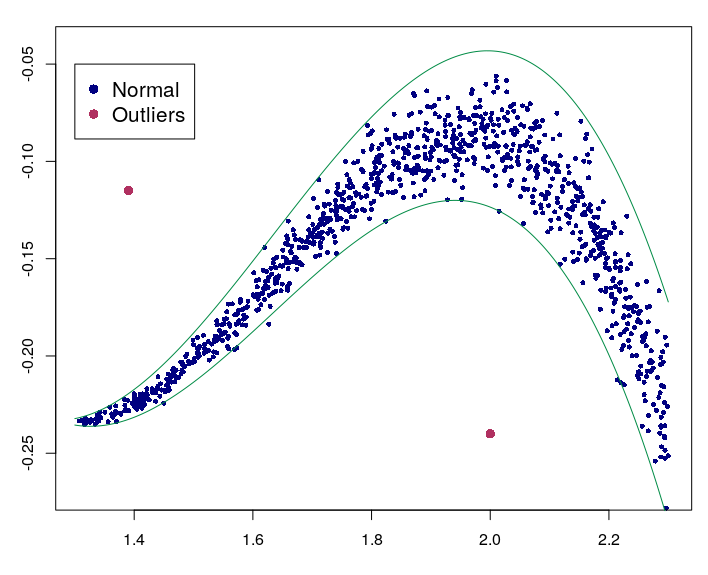
\includegraphics[width=\textwidth]{images/outlier_mine.png}
\caption{}
\end{subfigure}
\begin{subfigure}[b]{0.45\textwidth}
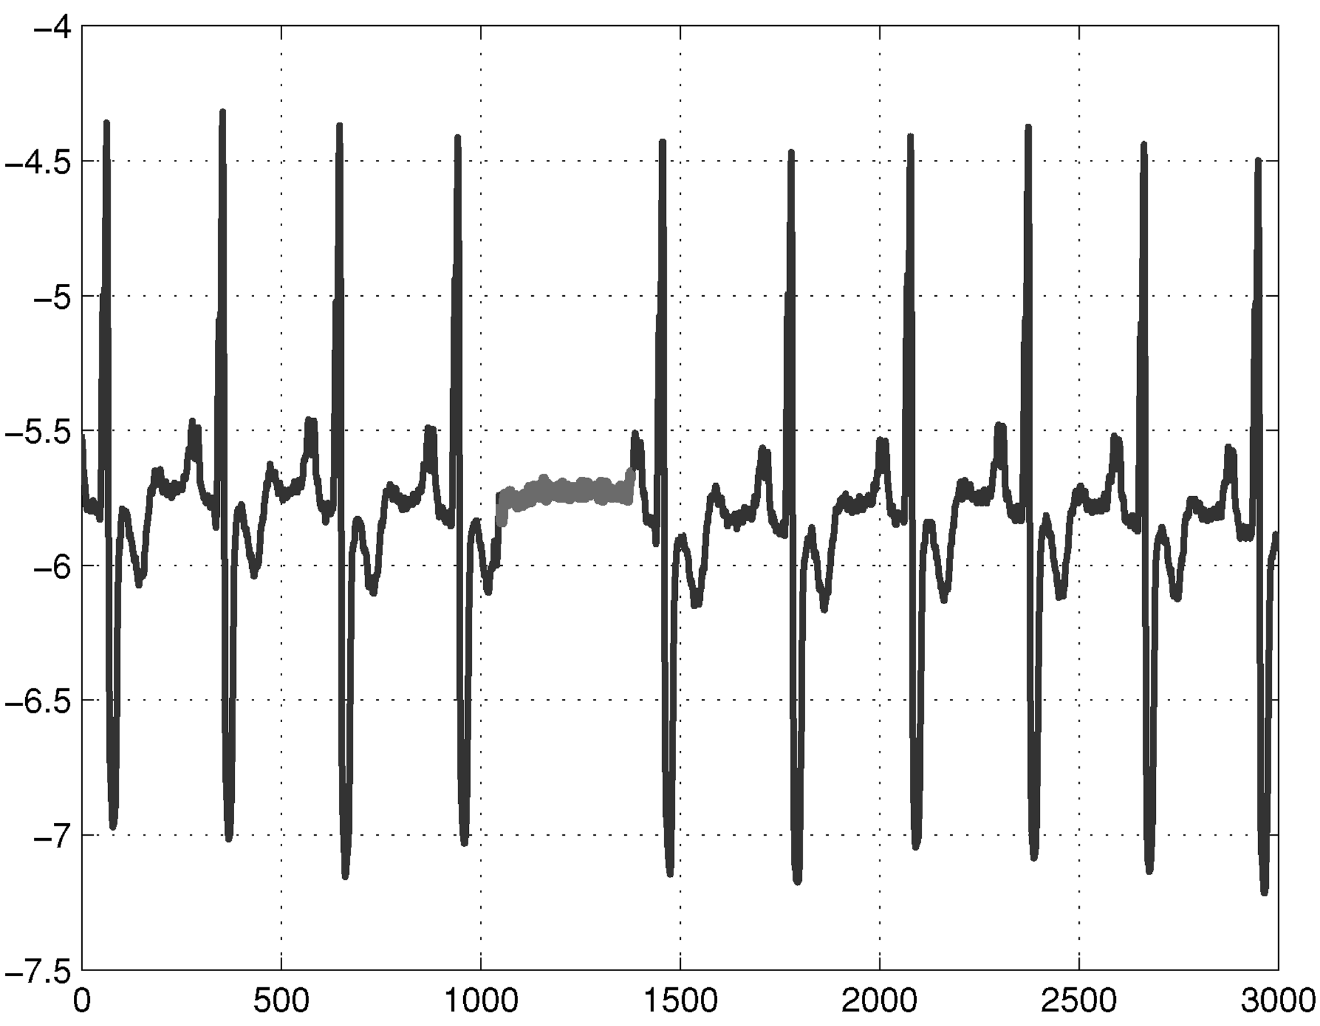
\includegraphics[width=\textwidth]{images/Atrial_Premature_Contraction.png}
\caption{}
\end{subfigure}
\caption{The left plot (a) depicts simple anomalies that deviate in distance from regular data. The right plot (b) shows a contextual anomaly where a group of data instances do not follow a repeating timely behaviour with respect to all other data points (corresponding to an \textit{Atrial Premature Contraction}, taken from \cite{chandola_anomaly_2009})}\label{graph2}
\end{figure}

Anomaly detection has found wide application in areas where stability of  critical systems or detection of their abuse is crucial. Examples of these include engine-fault detection in wind-turbines and fraud detection for credit cards. The assumption here is that the modelled system, such as the sensor-data stream of an engine or the buying behaviour of a customer, remains stable and generates consistent data. Detected anomalies in new observations then indicate a potential fault or abuse in this system. Obviously, it is not inherently clear that every abuse or fault generates data that differs from normal data. Therefore, it is important to choose data sources that are able to reflect the unique nature of a particular system.

\subsubsection{Anomaly detection and NIDS}

Anomaly detection has been applied to network security since the late 90's to assist IDSs. The behaviours of network computers are usually captured in the form of events logs such as network packets or flows, system calls, etc. The basic approach is to use collected training logs to infer a model of trustworthy activity, and then compare newly observed behaviour against this model.  To prevent any anomaly model from learning malicious behaviour as normal, the used training data has to be free of any attacks\footnote{Again, the assumption is that unauthorized and malicious activity will correspond to behaviour that differs from trustworthy one.}. 

As an example, an anomally large network flow involving an unusual pair of network computers could indicate that a hacked computer is extracting or sending out sensitive data to an unauthorized destination. An anomaly detection model does not make any assumptions about attack behaviour, but instead marks all deviations from the learned normal behaviour as potentially malicious. It is therefore better suited to find novel and unseen attacks. However, features mined from the data have to be able to reflect normal behaviour in a way that malicious traffic will look different in order to be detectable, which is not trivial. Furthermore, normal instances that only occur rarely or are diffuse will potentially also be flagged as potentially malicious, making an anomaly-based IDS prone to high false alert rates.


%\section{Controlling traffic and corresponding microstructures}
%\section{How traffic models are susceptible to microstructures}
%Include some of the findings from the stepping stone paper here:
%\begin{itemize}
%\item How models such as DeepCorr are set up to capture sequential dependencies
%\item How they are sucsceptible to chaff, long rtts, etc.
%\end{itemize}
%\subsection{Models that rely explicitely on microstructure modelling}
%Basically traffic classifiers
%\section{Application to intrusion-detection}
%\section{Capturing traffic microstructures on a flow-level with a bidirectional LSTM}
%\section{Capturing traffic microstructures on a packet-level with a LSTM-encoder}
%\section{Thesis plan}
%In the light of the problems described in Section \ref{Sec:Problems} that we encountered in the field of anomaly-based intrusion detection, I believe that the scope of this PhD-project has to be altered slightly. As there will not be enough material directly concerning anomaly detection, the formulation of building anomaly-detection models describing software behaviour should be relaxed to general applications of ML (not just anomaly detection) in specific areas related to software defined behaviour. 
%The overall unifying theme of this PhD so far has been centered around small-scale traffic structures generated by software-defined computer interactions and applications of ML language models to it, in other words \textbf{Modelling computer interactions as a language}.
%This could be based of the reoccurring use of traffic (and potentially system/program logs) generation for machine learning. The generated traffic could then be verified as valuable by the implemented intrusion detection applications.
%All applications implemented so far except for the flow-level model are driven (in part) by our traffic generation:
%\begin{itemize}
%\item Flow-level LSTM model
%\item stepping stone detection
%\item traffic relay
%\item LSTM encoder
%\item QUIC anomaly detection
%\end{itemize}
%Overall, all these applications except for the traffic relay detection are concerned with software-defined fine-grained structures. Below, I outline the different chapters that I believe should be included in my thesis:
%\begin{enumerate}
%\item Introduction and related work
%This chapter could largely draw from the existing introduction in the research proposal as well as the extensive literature survey I conducted. Updates on the scope as well as recent developments in related work would have to be added. %This should take less then three weeks.
%\item Background: Anomaly detection and challenges in security
%This chapter outlines the motivation to use anomaly-based detection models instead of classification-based ones. It furthermore highlights why anomaly detection is more difficult in security than in other areas, and what currently prevents it from being deployed outside of academia.
%\item Background: Language models and their application to security
%This chapter briefly outlines different techniques used in language modelling,  and how they can be used to build data representation useful for anomaly-detection. It also discusses previous applications of language models in security.
%\item Data sources, datasets, and data generation with realistic small scale structures
%This chapter will draw largely on the work conducted for the DetGen traffic generation framework.
%\item Computer communication structures and the effect of malicious behaviour on them
%This chapter will describe the different structures that the different layers of software-defined communication can have on the collected data. These descriptions and their corroboration can be taken from work in each of the projects described above. Furthermore, this chapter will describe how attacks can alter these structures due to the distinct approach they are taking, and why it is worth building models that focus on small-scale traffic structures.
%\item Traffic as a language and detection models
%This chapter will describe how network traffic can be described by a language model, and how to construct anomaly-based models from it. The chapter will then proceed to describe the different approaches I worked on and their respective results:
%\begin{enumerate}
%\item Flow-based modelling
%\item Connection setup model
%\item Traffic relating to process initialisations in the QUIC protocol
%\item Detecting similarity in computer connections
%\end{enumerate}
%\item Conclusions
%\end{enumerate}


\section{Temporal correlation/Semantics-based}

Despite network traffic being a stream of events, most anomaly-based intrusion detection approaches neglect any temporal features. Nevertheless, malicious behaviour most often is composed of  a series  of related computer and network  events and have a distinct temporal and semantic profile \cite{ye2000markov}. As an example, an intruder using a session relay to exfiltrate information or pass malicious code generates a strong dependency between incoming packets in one connection and outgoing packets in the other connection (and vice versa) albeit the individual packets or connections resemble perfectly benign behaviour\footnote{as they are essentially two normal connections that are relayed by the intruder}. Building a model that can that can understand relations and dependencies between individual events could potentially lead to great improvements in the detection of otherwise non-anomalous attacks. 

Since a machine's network traffic is the collective stream of multiple processes accessing the internet, individual traffic sequences are mixed with others, which makes the modelling of temporal dependencies a non-trivial task. In comparison to the other identified categories, research in the area of anomaly detection using temporal correlation or semantic models is sparse. 


In 2003, \textbf{Krishnamurthy et al.} \cite{krishnamurthy2003sketch} propose a rather simple, yet efficient method for network-wide monitoring of individual key occurrences in an online fashion. For that, a sliding window approach is used to asign all keys (which here stand for individual IP addresses or network ports) a value containing the number of its occurrency. For each key, the collected values are then used to train either an \textit{ARIMA} or a \textit{Holt-Winters} method, both popular and powerful time-series forecasting models which can be trained in an online fashion. Anomalies are then identified as values with a forecasting error exceeding a certain treshold and thus indicating a sudden change in occurrency-behaviour of that particular key. This is an improvement to summarisation measures such as entropy or histograms in two ways: It provides a better resolution of individual traffic channels, enabling the detection of attacks with far less volume, and enabling the modelling of more complex temporal patterns which become apparent on a lower level. And it makes attack attribution far simpler by indicating directly the key which is subject to an anomaly. 

Since traffic is usually arriving at a fast rate, it is a computationally hard and memory-consuming task to count the occurrencies of all keys simultaneously. Schweller et al.  overcome this problem using a \textit{sketch-based counting approach} which uses hash-function to direct the values of a key directly to a position in a hash table without the need to store actual key in the memory. As this process is not exact, the count value is subject to statistical variations and the authors propose an unbiased estimator. The inaccuracy of the count estimator is also preventing the authors from using a probabilistic approach to anomaly detection instead of simple tresholding. However, this approach is also only counting occurrencies and does not detect any correlated key behaviour.

A great problem of the proposed framework is the fact that the key translation works only in one direction, making it impossible to associate a detected change with the corresponding key. This problem is overcome by \textbf{Schweller et al.} \cite{schweller2004reversible} who propose a reversible sketch method.

\textbf{Pellegrino et al.} \cite{pellegrino2017learning} last year proposed \textit{BASTA}, a framework to mine behavioural fingerprints from network flows using \textit{timed automata learning}. An automata encodes patterns of short-term interactions of a system and is a representation of symbolic sequences, often corresponding to state transitions, which it encodes in a state transition function. Applied to network flows, an automata represents sets of events\footnote{distinguished by port,  protocol, etc.} that can follow each other in the network trace of a system. To be more specific, they used a type of probabilistic automata that works with transition probabilities and thus works in a similar way to a \textit{hidden Markov model}. Events are asigned a state corresponding to the protocol and the direction of the flow, and the quantile\footnote{of the overall distribution of the individual parameters} its duration, size, and number of packets are lying in. The authors then use this framework to create malicious fingerprints by training it on malicious traffic intermixed with normal traffic. These fingerprints are then detected on an infected host if the difference between the expected and the observed state counts drops below a treshold. 

This paper is itself not developing any anomaly detection techniques, and I will not discuss the flaws of its application for malware fingerprinting. It is interesting for us as the developed automata mining techniques can also find direct application in mining normal behaviour automata and thus be used in an anomaly detection model. 


\textbf{Noble and Adams} \cite{noble_real-time_2018, noble_correlation-based_2016} have recently proposed \textit{ReTiNa}, a tool that measures temporal changes in the correlation between individual events in order to find intrusions on individual hosts. In their approach, they estimate the correlation between the time passed between two events, also called \textit{interarrival time}, of an OD pair and the associated size or number of packets of the involved events. For this, interarrival time and the size/packet number are modelled as a bivariate gaussian distribution, and the covariance matrix is estimated using maximum-likelihood-estimation. The authors use a sophisticated online-estimation method to adapt the estimates to changes in the correlation structure, which can then be identified by comparison to an offline estimate. Anomalies are then identified as a collection of changes happening across multiple OD pairs on one host or in the entire network by simple hypothesis testing, which decreases the false-positive rate. The assumption here is that different OD pairs are independent of each other.


A big advantage of this approach is that it is adaptive and does not need a training phase, i.e. it is not reliant on attack-free training data. The method was tested both on the LANL network flow data as well as internal data from the \textit{Imperial College Academic network}. The method found several anomalies that coincide malicious activity in the network, but a definitive conclusion whether they are related is difficult to make.

\textbf{Whitehouse, Evangelou and Adams} \cite{whitehouse_activity-based_2016} modeling the number of 
network flow and \textit{user authentication} events on individual hosts as a polynomial function of the time and day and its rarity. Anomalies are then identified using Fisher's product test statistic and the reconstruction error. The method was tested on the LANL data using the auth and the flow sources and wa able to identify persistent structures in the data. 


\subsection{Application to stepping stone detection}

Especially in larger computer networks, attackers often try use relay-like command chains, also called \textit{stepping stones}, to obfuscate their origin or access machines without external connection. In such a chain, no direct connection exists between the first and the last machine, commands are sent through one or multiple intermediate machines. Stepping stone connections are usually encrypted and are notoriously difficult to identify. Upon detection, pairs of stepping stones are a clear indication of anomalous activity. 

As stepping stone detection falls much more in the field of misuse detection, I will only give a very brief overview over emplyed techniques.

\textbf{Zhang and Paxson} \cite{zhang2000detecting} proposed one of the first methods for detecting stepping stones in 2000. They model relayed key-stroke packet streams as a two-dimensional ON/OFF switching process, where state changes have to occur within a certain window between the two channels. Correlation is then simply detected if the number of switches lying in this window exceeds a treshold. 


A common assumption made when trying to find stepping stones is that packet or flow streams between different hosts in a network are almost always independent of each other, which is shown by \cite{neil2013scan}. \textbf{He and Tong}\cite{he2007detecting} model normal packet arrivals in a connection as a Poisson Process, and use the assumption of independence to derive a probabilistic distribution for the similarity of packet numbers in two channels in a time interval. P-values are then used to identify when the number of similar intervals becomes unlikely. They also show that if the ratio of chaff-packets exceeds to necessary packets in a stepping stone becomes too large, correlation is impossible to detect under the asumption of normal traffic following a Poisson distribution.


\textbf{Neil et al.}  \cite{neil2013scan} also model normal event arrivals along an edge as a \textit{negative Binomial process} with two different rates, evolving as a hidden Markov model, and correlation in different time intervals in then used  using a likelihood ratio test to obtain p-values. In their approach, instead of testing network wide correlation, which is computationally unfeasible, testing is done on two different forms of local subgraphs, a star shape and a path-shape on selected edges. 


\subsection{Semantic-based approaches using different data sources}

Approachs that model semantic or temporal behaviour characteristics have been also been applied on host-based data streams such as \textit{system call logs} or \textit{process logs} as well. As these are mostly symbolic event streams, anomaly detection in principal works similarly as for network traffic. As these data sources have usually a more hierarchical structure of events following each other in a parent-child fashion and therefore do not suffer from overlapping signals, and it is generally easier to identify semantic structures. Notable examples include the use of deterministic automata \cite{warrender1999detecting}, Markov chains \cite{ye2000markov}, hidden Markov models \cite{yeung2003host,hu2009simple}, or \textit{recurrent neural networks}\cite{du2017deeplog}.


\section{Existing datasets}

In order to evaluate their ability to model the behaviour of a network and to identify malicious activity and network intrusions, new methodologies have to be tested using existing datasets of network traffic. This network should ideally contain realistic and representative benign network traffic as well as a variety of different network intrusions. However, as  network traffic contains a vast amount of information about a network and its users, it is notoriously difficult to release a comprehensive dataset without infringing the privacy rights of the network users. 
Furthermore, the identification of malicious traffic in network traces is not straightforward and often requires a significant amount of manual labelling work.
For that reason, only a handfull of datasets for network intrusion datasets containing real world traffic exist. There have also been some efforts to artificially creating such datasets and thus bypassing any privacy concerns. However, up to today, no artificial dataset truly resembles real network traffic in every aspect \cite{nisioti2018intrusion}.

As described in a recent survey by \textbf{Ahmed et al.} \cite{ahmed2016survey}, we can generally distinguish four different types of datassets containing network traffic:

\begin{enumerate}

\item \textbf{Real network data containing known intrusions}: 

\item \textbf{Real network data containing injected intrusions}:

\item \textbf{Real network data containing no intrusions/untruthed real network data}:

\item \textbf{Synthetic network data with/without injected intrusions}:

\end{enumerate}

I will now describe the properties of existing datasets suitable for network intrusion detection. As this review is primarily concerned with anomaly detection models that require benign network traffic, I did not include datasets such as honeypots that mostly contain malicious traffic. A description that includes such datasets can be found in the below described survey by Ahmed et al. \cite{ahmed2016survey}.



\subsubsection*{Los Alamos National Laboratory, 2015 - Comprehensive, Multi-Source Cyber-Security Events \cite{akent-2015-enterprise-data}\cite{kent-2015-cyberdata1}}

In 2015, the Los Alamos National Laboratory (LANL) released a large dataset containing \textbf{network flow} traffic from teir corporate computer network, which contains about 17600 computers. The data was gathered over a period of 58 days with about 600 million events per day. The data only contains internal network connections, i.e. no flows going to or coming from computers outside the network are included. IPs and ports were de-identified (with the exception of the most prominent port), but are consistent throughout the data. Since the data stems exclusively from one corporate network, it can be assumed that it shows more homogeneity in the observed traffic patterns than  general network traffic.

Additionally, the dataset also contains other event sources which were recorded in parallel in order to give a more comprehensive look at the network, and could be very useful when investigating a detection approach that correlates multiple event sources. These sources include process events and authentication events from Windows-based computers and servers, and DNS lookup events from the DNS servers within the network. 

The dataset furthermore contains a labeled set of redteam events which should resemble intrusions. However, these events are not part of the network flow data and only contain information about the time of the attack and the attacked computer. These events apparently resemble remote \textit{access attacks}, are not described further and appear to be artificial or injected into the dataset. It is thus not certain how well they resemble actual network intrusions.


LANL released another dataset containing network flow traffic from their network in 2017 \cite{turcotte17}. This dataset is similar to the one from 2015, but spans over a longer period of time, 90 days. Furthermore, it contains no labeled malicious activity,  however that does not mean that the data is completely free of malicious activity.

\subsubsection*{CTU 2013 \cite{noauthor_ctu-13_nodate, garcia2014empirical}}

The \textit{Stratosphere Laboratory} in Prague released this dataset in 2013 to study botnet detection. It consists of more than 10 million labeled \textbf{network flows} captured on lab machines for 13 different botnet attack scenarios. Additionally, the raw packets for the botnet activity is also available for attack analysis. 

The labelling in this dataset is different from other datasets as each  flow  in  the  list  is  labeled  based  on  the  source  IP  address.  In  the experiments,  certain  hosts  are  infected  with  a  botnet  and  any  traffic  arising from such a host is labeled as Botnet traffic. Traffic from uninfected hosts is labeled as Normal. All other traffic is Background, as one cannot classify it. 

A criticism of this dataset is the unrealistically high amount of malicious traffic contained in the dataset, which makes it easier to spot it while reducing false positives. Furthermore, the way normal or background traffic is generated is described only poorly and leaves the question how representative it is of actual network traffic.

\subsubsection*{UGR 2016 \cite{macia2018ugr}}

The UGR'16 dataset was released by the University of Grenada and contains \textbf{network flow}\footnote{netflow v9} data from a spanish 3-tier ISP. This ISP is a cloud service provider to a number of companies, and thus the data comes from a much less structured network than the LANL data. It contains both client's access to the Internet and traffic from servers hosting a number of services. The data therefore contains a very wide variety of traffic patterns, an advantage emphasised by the authors. IP-adresses are consistently anonymised while network ports are unchanged. However, it is not ensured that the traffic capture is complete, i.e. that all traffic coming from and going to a particular machine is captured.

A main focus in the creation of the data was the consideration of long-term traffic evolution and observable periodicity in order to enable the testing of so called \textit{cyclostationary} traffic models. The dataset correspondingly covers a very long period, spanning from March to August of 2016, and containing about 14 GB of traffic per week. 

The data is split into a training set and a test set, with the latter containing labeled attack data. This attack data does not stem from rogue agents but is in part generated in controlled attacks on victim machines, and in part injected from previously observed malware infections. The attack data is therefore does not truly correspond to actual attacks, but achieves a high degree of similarity. The implemented attacks contain:
\begin{itemize}
\item DoS attacks (controlled attacks),
\item Port scanning (controlled attacks),
\item C\&C traffic from a botnet (injected).
\end{itemize}

The authors also acknowledge that the background traffic is not necessarily free from further attacks. In fact, three real attacks have been observed and labeled, corresponding to IP-scanning and a spam mail campaign.

\subsubsection*{UNSW-NB 2015 \cite{moustafa_unsw-nb15:_2015}}

The dataset realeased by the \textit{University of New South Wales} in 2015 contains real background traffic and synthetic attack traffic collected at the "Cyber Range Lab of the Australian Centre for Cyber Security". The data is collected from a small number of computers which generate real background traffic, and is overlayed with attack traffic using the \textit{IXIA PerfectStorm tool}. The time span of the collection is in total 31 hours.

An advantage of the collected dataset is the inclusion of both \textbf{raw packets} and \textbf{network flows} along with two other data formats containing newly engineered features. This allows a more detailed analysis of the data and possibly a better distinction between attack and benign traffic. In total, the data contains 260 000 events.

Another advantage of the data is the variety of attack data, containing a number of DoS, reconnaissance, and access attacks. However, due to the synthetical injection of these attacks, it is unclear how close they are to real-world attack scenarios.

Since this dataset is collected from a relatively small number of machines and during a limited period of time, it is furthermore unclear how suitable for capturing both the temporal evolution and the heterogeneity of real background traffic.

\subsubsection*{CICIDS 2017/2018 \cite{gharib2016evaluation}\cite{sharafaldin2018towards}}

This dataset, released by the \textit{Canadian Institute for Cybersecurity} (CIC), contains 5 days of network traffic from 12 computers. These computers all have either different different operating systems such as Windows, OSX, or Ubuntu, or different versions of the same operating system in order to enable a wider range of attack scenarios. The network  furthermore contains switches, routers, a web server, a modem, and a firewall in order to ensure a realistic network topology. The traffic data itself consists of \textbf{labeled benign and attack traffic}, and is available as 11 GB per day of \textbf{raw packets} with payloads, or as \textbf{network flows}. 

It was ensured that the data contains all traffic coming and going from individual machines. However, in contrast to other datasets, the background traffic is not directly generated through user interactions on the machine, but by using a method to profile abstract user behaviour in different traffic protocol. The purpose of this is to make the traffic more heterogenuous and to ensure that different types of behaviour are present in the data during the comparably short time span. This  However, it is not completely clear how much of the underlying structure of real traffic is lost in the process, and therefore how suitable this data is to build models of benign user activity.

The attack data of this dataset is one of the most diverse among NID datasets, as it contains a variety of up-to-date attacks, such as different types of DoS attacks, SQL-injections and Heart-bleed attack, network scanning, or botnet activity. These are not always successful in order to reflect actual attack scenarios. However, the authors did not describe very well how the data from these attacks is generated and combined with the background traffic as it is also processed through a form of profiling engine. 

\textbf{CICIDS 2018:}
This dataset is generated in a similar fashion to the CICIDS 2017 data that we used in this work. The main differences are that the CICIDS 2018 data spans over three weeks and includes in total 450 hosts, but lacks the amount of web-attacks that we require and which is present in the CICIDS-2017 dataset.

The CIC released another very similar dataset to these ones in 2012.

\subsubsection*{DARPA 1998 \cite{lippmann2000evaluating}}

The \textit{Defense Advanced Research Projects Agency} released the first major dataset to test network intrusion detection systems. The data stems from two experiments at the \textit{MIT Lincoln Laboratory} were multiple victim hosts running Unix and Windows NT were subject of over 200 attacks of 58 different types. The data spans three weeks of training and two weeks of testing data and contains \textit{raw packets} that are labeled. It was since then heavily used as a benchmark to test new detection methods. %In 2000, the original data was post-processed to reduce some of its shortcomings.

Also due to its prominence, it was heavily scrutinised and received a lot of criticism for its lack of realistic background traffic, which was generated through simulation procedure, and the presence of artifacts from these simulations in the data that could heavily skew any model relying on benign traffic. Also, the high percentage of attack traffic in the data is described as unrealistic.

Furthermore, since the dataset is now more than 20 years old, it is remarked that both the benign and attack traffic does not resemble modern network traffic anymore. 

\subsubsection*{KDD Cup 1999 \cite{cup1999data,cup1999dataset}/NSL-KDD 2012 \cite{tavallaee2012nsl}}

The \textit{MIT Lincoln Laboratory} created this dataset in 1999 by processing portions of the 1998 DARPA dataset with new labels for a competition at the conference on \textit{Knowledge Discovery and Data Mining}, and is the most widely used dataset in intrusion detection. It contains 2 million connections summaries in a new format and in total 38 attack types. This new format is essentially a form of \textbf{network flows} with a greatly increased number of features, 46 in total, which give additional details about the origin of the connection. The availability of these features in a real-world application however is in my opinion unrealistic as most of them could be mined due to the availability of parallel surveilance of the host, a Solaris-based system. However, we can see significant differences in today's operating systems which barely resemble Solaris. In addition, parallel host system surveilance usually cannot be taken for granted in a realistic network environment. Naturally, as the KDD'99 data stems directly from the DARPA dataset, it also faces the same problems and criticism. 

The \textit{Canadian Institute for Cybersecurity} postprocessed the KDD'99 data in order to address some of its shortcomings. This includes removing redundant records, balancing the size of the training and test data, and adjusting the proportion of attack traffic in the data. However, the biggest criticism from the KDD'99 and the DARPA data, the unrealistic generation of background data, still prevails.

\subsubsection*{LBNL 2013 \cite{pang2005first}}

This dataset released by the \textit{Lawrence Berkeley National Laboratory} in 2005 is the first one to examine internal network traffic inside a modern enterprise. It contains more than 100 hours of \textit{packet headers} from several thousand internal hosts. 

This dataset contains no known attack traffic, and is therefore only suitable for traffic analysis and model fitting analysis. Furthermore, as being the first dataset containing enterprise traffic, privacy concerns caused the authors to remove any possibilities to identify individual IP addresses.

In 2011, Saad et al. \cite{saad2011detecting} combined this dataset with existing botnet traffic to create a dataset containing both benign and attack traffic. 

\subsubsection*{UNIBS 2009\cite{UNIBS2009data}}

This dataset was collected on the campus network of the \textit{University of Brescia} on three consecutive days in 2009. The dataset contains in total 79000 anonymised TCP and UDP \textit{network flows}. 

This dataset is not directed towards intrusion detection research, but was made as \textit{ground truth data} for traffic classification. It therefore contains labels which indicate which of in total six applications generated the corresponding traffic flow. It might however still be of interest for model assessment in intrusion detection that is relying on traffic classification.

\subsubsection*{CAIDA 2016 \cite{walsworth2015caida}}

The \textit{Center for Applied Internet Data Analysis} started collecting network traces from a high-speed backbone link in 2008 with the collection still ongoing. The data is available in anonymised yearly datasets containing one hour of \textbf{packet headers} for each month. 

Since the traffic is collected from a backbone link, it is very unstructured and heterogenuous. It is furthermore not necessarily free from attack traffic. Although this dataset has been used for intrusion detection before, it is more suitable for general internet traffic analysis.


\subsubsection*{MAWI 2000 \cite{sony2000traffic}}

Similarly to the CAIDA dataset, this dataset contains \textbf{packet headers} from the WIDE backbone. It is therefore similarly unstructured, anonymised, and not free from attack traffic. Since this dataset was already collected and released in 2000, it can also be remarked that the contained traffic is too old to represent modern traffic. 

\subsubsection*{ADFA 2013/2014 \cite{creech2014developing,creech2013generation}}

The ADFA datasets, released by the \textit{University of New South Wales}, focuses on attack scenarios on Linux and Windows systems as well as \textbf{stealth attacks}. To create host targets, the authors  installed web servers and database servers , which were then subject to a number of attacks. 

The dataset contains both attack traffic and benign traffic. However, the dataset is directed more towards attack scenario analysis and is criticised as being unsuitable for intrusion detection due to its lack of traffic diversity. Furthermore, the attack traffic is not well separated from the normal one.

\subsubsection*{ICT datasets \cite{USC2010ICT}}

The \textit{Impact Cyber Trust} releases cyber security oriented data. Its repository includes many datasets, synthetic as well as real captures, from different sources. Many datasets focus on observed attack data and thus are not directly applicable to intrusion detection. Furthermore, there is in general very little information provided that describes a dataset's origin, which makes it hard to investigate the network topology.

Among the more useful datasets are the \textit{USC datasets}\footnote{DS-062, LANDER Data, and DS-266}, which contain network traffic (both \textbf{packet headers} and \textbf{network flows}) from academic networks in the US between 2008 and 2010. The datasets are very large, with the largest one covering 48 hours and containing 357 GB of packet headers. 

\subsubsection{LITNET-2020 \cite{damasevicius2020litnet}}

The LITNET-2020 from the Kaunas University of Technology Lithuania from 2020 was collected from an academic network over a timespan of 10 months and contains annotated real-life benign and attack traffic. The corresponding network provides a large network topology with more than a million IP-addresses, and the data was collected in the form of network flows with more than 80 features. However, the dataset only contains traffic from high volume attacks such as DoS-, scanning, or worm attacks, which are not suitable to evaluate CBAM.

\subsubsection{Bo{\u{g}}azi{\c{c}}i University distributed denial of service dataset} \cite{erhan2020bougazicci}

The Bo{\u{g}}azi{\c{c}}i University distributed denial of service dataset contains both benign traffic from more than 400 users from an academic network as well as artificially created DoS-attack traffic. The dataset spans only 8 minutes and contains no access attacks.



